\section{Kết quả}

\subsection{Đường cong học tập}

Quá trình huấn luyện baseline được tóm tắt ở Bảng~\ref{tab:lich-su-huan-luyen}. Có thể thấy rõ hai pha: Trong ba epoch đầu, val loss giảm đồng pha với train loss, phản ánh quá trình học có ý nghĩa. Từ epoch 4 trở đi, train loss tiếp tục giảm sâu nhưng val loss quay đầu tăng, dấu hiệu rõ ràng của quá khớp (overfitting). Mô hình tốt nhất được giữ lại tương ứng với epoch 3, nơi val loss đạt $0,3042$ và val accuracy đạt $0,8776$.

\begin{table}[htbp]
\centering
\caption{Lịch sử huấn luyện baseline. Epoch tốt nhất được in đậm.}
\label{tab:lich-su-huan-luyen}
\begin{tabular}{ccccc}
\hline
\textbf{Epoch} & \textbf{Train loss} & \textbf{Train acc} & \textbf{Val loss} & \textbf{Val acc} \\ \hline
1              & 0,4778              & 0,7742             & 0,3510            & 0,8612           \\
2              & 0,2712              & 0,8964             & 0,3577            & 0,8408           \\
\textbf{3}     & \textbf{0,1893}     & \textbf{0,9302}    & \textbf{0,3042}   & \textbf{0,8776}  \\
4              & 0,1268              & 0,9553             & 0,3817            & 0,8764           \\
5              & 0,0791              & 0,9731             & 0,4194            & 0,8688           \\ \hline
\end{tabular}
\end{table}

Hình~\ref{fig:duong-cong-learning} minh họa trực quan diễn biến này. Đường val loss (cam, biểu đồ trái) chạm điểm thấp nhất tại epoch 3 rồi quay đầu đi lên, trong khi val accuracy (cam, biểu đồ phải) đạt cực đại tại cùng epoch và sau đó dao động nhẹ quanh $0,87$. Đường train (xanh) tiếp tục cải thiện đơn điệu trên cả hai tiêu chí, hình thái kinh điển của hiện tượng quá khớp khi mô hình bắt đầu ghi nhớ chi tiết của tập huấn luyện.

\begin{figure}[htbp]
    \centering
    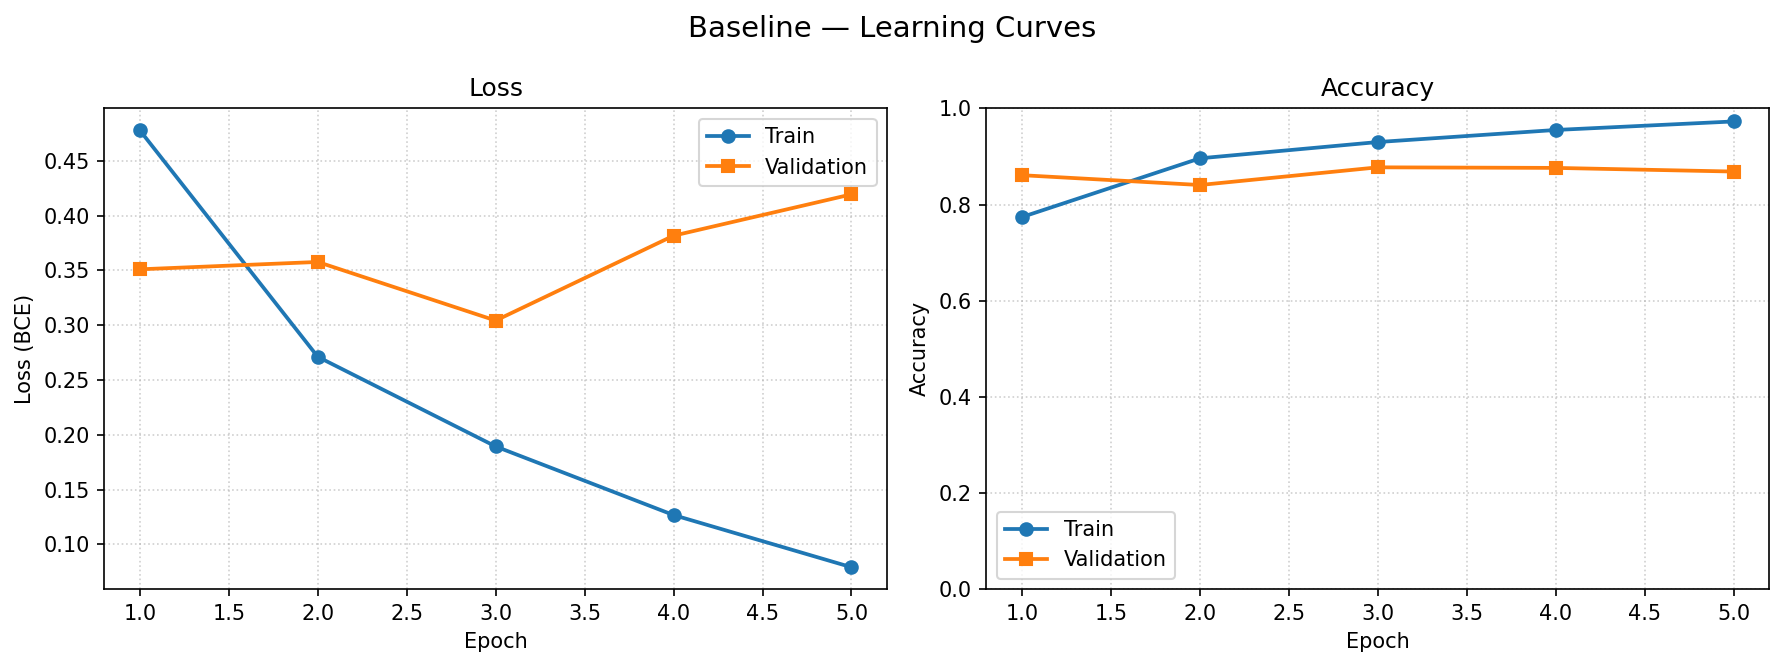
\includegraphics[width=0.9\textwidth]{figures/baseline_learning_curves.png}
    \caption{Đường cong loss (trái) và accuracy (phải) của baseline trên tập huấn luyện so với tập validation qua năm epoch. Điểm gãy ở epoch 3 đánh dấu khởi đầu của giai đoạn quá khớp.}
    \label{fig:duong-cong-learning}
\end{figure}

Khoảng cách giữa train accuracy và val accuracy ở epoch 5 lên tới $0,1043$, một mức khá đáng kể, chứng tỏ mô hình bắt đầu ghi nhớ dữ liệu huấn luyện. Cơ chế chốt mô hình theo val loss thấp nhất đã thực hiện đúng vai trò của nó: kết quả test cuối cùng được đánh giá trên trạng thái epoch 3 chứ không phải epoch 5 với train accuracy cao hơn.

\subsection{Đánh giá trên tập kiểm thử}

Mô hình tốt nhất theo val loss được đánh giá trên $25\,000$ mẫu kiểm thử và đạt độ chính xác $0,8697$. Bảng~\ref{tab:do-do-kiem-thu} trình bày bốn độ đo chính cùng tổng hợp theo lớp.

\begin{table}[htbp]
\centering
\caption{Độ đo trên tập kiểm thử ($25\,000$ mẫu).}
\label{tab:do-do-kiem-thu}
\begin{tabular}{lcccc}
\hline
\textbf{Lớp} & \textbf{Precision} & \textbf{Recall} & \textbf{F1} & \textbf{Số mẫu} \\ \hline
Tiêu cực     & 0,8613             & 0,8814          & 0,8712      & $12\,500$       \\
Tích cực     & 0,8786             & 0,8580          & 0,8682      & $12\,500$       \\ \hline
Macro avg    & 0,8699             & 0,8697          & 0,8697      & $25\,000$       \\ \hline
\end{tabular}
\end{table}

Hai lớp có độ đo gần như cân bằng, không có hiện tượng mô hình thiên về một phía. Tuy nhiên, recall của lớp tích cực ($0,8580$) thấp hơn precision ($0,8786$), cho thấy mô hình hơi bảo thủ khi dự đoán positive: nó bỏ sót một số bài đánh giá thực sự dương nhiều hơn là tạo ra cảnh báo dương sai. Sự bất đối xứng này được phản ánh trực tiếp trong ma trận nhầm lẫn ở Bảng~\ref{tab:ma-tran-nham-lan}.

\begin{table}[htbp]
\centering
\caption{Ma trận nhầm lẫn trên tập kiểm thử.}
\label{tab:ma-tran-nham-lan}
\begin{tabular}{lccc}
\hline
                  & \textbf{Dự đoán tiêu cực} & \textbf{Dự đoán tích cực} & \textbf{Tổng} \\ \hline
\textbf{Tiêu cực thật} & $11\,018$                  & $1\,482$                   & $12\,500$     \\
\textbf{Tích cực thật} & $1\,775$                   & $10\,725$                  & $12\,500$     \\ \hline
\textbf{Tổng}          & $12\,793$                  & $12\,207$                  & $25\,000$     \\ \hline
\end{tabular}
\end{table}

Hình~\ref{fig:confusion-matrix-normalized} trình bày dạng chuẩn hóa theo hàng của ma trận này, giúp đọc trực tiếp recall trên mỗi lớp: lớp tiêu cực đạt recall $0,881$ (mô hình bắt đúng $88,1\%$ mẫu negative), trong khi lớp tích cực đạt recall $0,858$. Khoảng cách hai phần trăm này phù hợp với mật độ false negative cao hơn đã ghi nhận ở Bảng~\ref{tab:ma-tran-nham-lan}.

\begin{figure}[htbp]
    \centering
    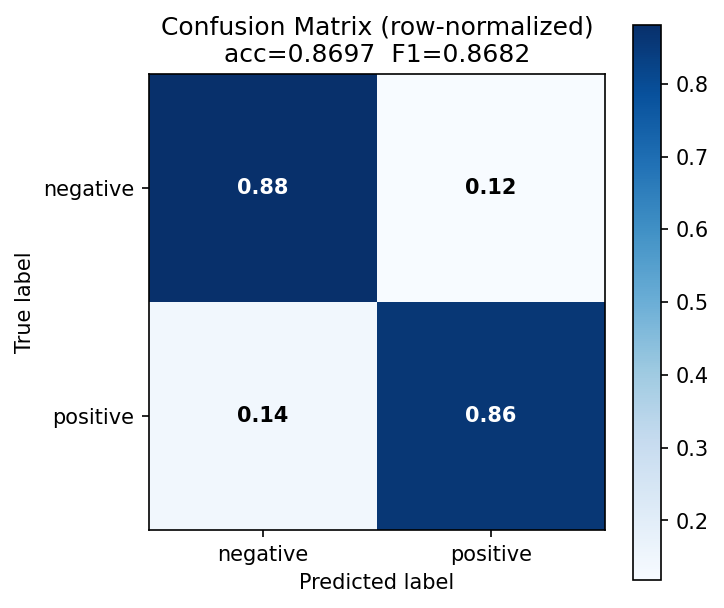
\includegraphics[width=0.5\textwidth]{figures/confusion_matrix_normalized.png}
    \caption{Ma trận nhầm lẫn chuẩn hoá theo hàng. Đường chéo chính là recall
của mỗi lớp.}
    \label{fig:confusion-matrix-normalized}
\end{figure}

Tổng số dự đoán sai là $3\,257$, ứng với tỉ lệ lỗi $13,03\%$. Trong đó, $1\,482$ trường hợp là false positive (mô hình gán nhãn tích cực cho một bài đánh giá thực sự tiêu cực) và $1\,775$ trường hợp là false negative (mô hình gán nhãn tiêu cực cho một bài đánh giá thực sự tích cực). Sự lệch nhẹ về phía false negative củng cố nhận xét ở đoạn trên.

\subsection{Phân tích các trường hợp dự đoán sai}

Xét các trường hợp dự đoán sai có độ tự tin cao nhất, những trường hợp mang nhiều thông tin chẩn đoán hơn cả cho hệ thống. Phía \textit{false positive}, mẫu khiến mô hình tự tin nhất ($p = 0,9997$) là một bài đánh giá tiêu cực nhưng lại được viết bằng giọng kể chuyện hài hước, sử dụng nhiều từ ngữ mang sắc thái tích cực ở bề mặt theo nghĩa châm biếm. Một mẫu \textit{false positive} tiêu biểu khác ($p = 0,9984$) thực chất lại là một bài đánh giá tích cực rất rõ ràng nhưng bị gán nhãn sai thành tiêu cực trong tập dữ liệu gốc, một hiện tượng nhiễu nhãn hệ thống đã được ghi nhận trên nhiều bộ dữ liệu chuẩn (\textit{benchmark}) nổi tiếng bởi Northcutt và cộng sự (2021). Ở chiều ngược lại của phía \textit{false negative}, mẫu dữ liệu mà mô hình tự tin sai nhất ($p = 0,0010$) là một bài đánh giá tích cực về một bộ phim khoa học viễn tưởng có nội dung tăm tối; tác giả sử dụng hàng loạt từ ngữ mang sắc thái tiêu cực để miêu tả bối cảnh và các cảnh phim nhưng lại đi đến kết luận ủng hộ ở cuối bài. Trong trường hợp này, mô hình đã bị chi phối hoàn toàn bởi mật độ quá cao của các từ tiêu cực bề mặt mà không thể nắm bắt được cấu trúc đảo chiều ngữ cảnh.

Tổng hợp lại từ các phân tích định tính trên, ta nhận diện được bốn nhóm nguyên nhân lỗi chính của kiến trúc hiện tại. Thứ nhất là hiện tượng châm biếm và cảm xúc trộn lẫn, xuất hiện khi cấu trúc bề mặt của ngôn ngữ mâu thuẫn hoàn toàn với ý nghĩa cốt lõi thực sự. Thứ hai là lỗi cắt cụt thông tin do giới hạn cấu hình $256$ token, thường xảy ra ở các bài đánh giá dài mà tín hiệu cảm xúc quyết định lại nằm ở phần kết luận. Thứ ba là những bài đánh giá quá ngắn nhưng chứa các từ gợi ý (\textit{cue}) đơn lập mạnh, khiến mô hình dễ rơi vào trạng thái tự tin thái quá. Cuối cùng là vấn đề nhãn sai trong tập dữ liệu gốc, một loại lỗi hệ thống không thể khắc phục bằng việc nâng cấp hay tối ưu hóa cấu trúc mô hình mà chỉ có thể giải quyết thông qua các quy trình lọc và làm sạch dữ liệu chuyên sâu.